\begin{frame}
\frametitle{Improvements?}
\begin{itemize}
\item Entropy \& information gain not sufficient metrics
\vfill
\item Missing data has to be handled
\vfill
\item Numerical values could provide order or dimension to a problem set
\vfill
\item Tree can be simplified
\end{itemize}
\end{frame}

\begin{frame}[allowframebreaks]
\frametitle{Missing data}
\begin{center}
%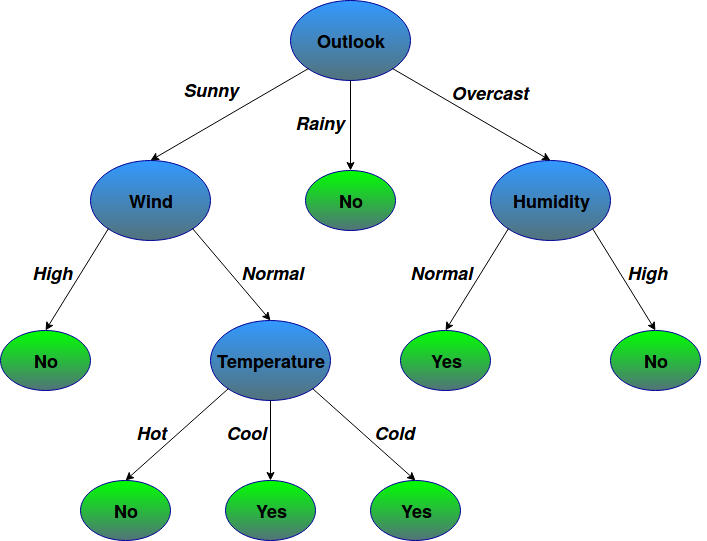
\includegraphics[scale=.1]{Images/DecisionTree.png}

2,*,*,*,*,*,2\\
1,2,*,*,*,*,1\\
1,1,2,*,*,*,1\\
1,1,1,*,*,*,1\\
1,1,3,2,2,*,1\\
1,*,*,*,*,4,1\\
2,1,4,*,*,1,1\\
2,1,4,*,*,2,1\\
2,1,4,*,*,3,1\\
2,1,3,1,1,1,1\\
2,1,3,1,1,2,1\\
2,1,3,1,2,1,1\\
2,1,3,1,2,2,1\\
1,1,3,1,1,3,1\\
2,1,3,1,2,3,1
\end{center}

\begin{itemize}
\item Dataypes can co-exist (eg. strings, integer/float)
\vfill
\item Solutions
\begin{itemize}
\item Replace missing values in column with most frequent
\item For numerical values replace with mean/mode/median
\end{itemize}
\item Column 2:
\begin{itemize}
\item No instances = 15
\item Card(2) = 1
\item Card(1) = 12
\item $\rightarrow$ safest choice replace missing values with 1 
\end{itemize}
\item Column 3:
\begin{itemize}
\item No instances = 15 (of course)
\item Card(2) = 1 
\item Card(1) = 1
\item Card(3) = 7
\item Card(4) = 3
\item Missing = 3
\item $\rightarrow$ replace missing values with 3
\end{itemize}
\end{itemize}
\end{frame}

\begin{frame}
\frametitle{Numerical \& continuous variables}
\begin{itemize}
\item General approach separate categorical and continuous
\vfill
\item Our implementation:
\begin{itemize}
\vfill
\item Treat all numerical variables as continuous
\vfill
\item C45 implementation based on  a binary tree (computational gain)
\vfill
\item $\rightarrow$ Everything equal or smaller than node value to the left
\vfill
\item $\rightarrow$ Everything else to the right
\end{itemize}
\end{itemize}
\end{frame}




\begin{frame}[allowframebreaks]
\frametitle{C4.5}
\begin{itemize}
\item Simplifying a tree
\vfill
\begin{itemize}
\item Given a target gain level (generic or user-defined)
\vfill
\item Prune (condense) the subtree
\vfill
\begin{itemize}
\item Might induce overclassification or errors
\vfill
\item Decreases the depth of the tree 
\vfill
\end{itemize}
\end{itemize}
\item 2 strategies:
\vfill
\begin{itemize}
\item \textbf{Pre-prune:}
\vfill
\begin{itemize}
\item Using statistical signifiance
\vfill
\item $\rightarrow$ stop growing/building when no statistical significant association between any attribute and class at a node
\vfill
\item chi-squared test ( too much statistics for us)
\vfill
\item Pre-pruning may stop growing prematurely (eg. XOR stops at root node)
\vfill
\end{itemize}
\framebreak
\item \textbf{Post-prune:}
\begin{itemize}
\item Subtree replacement
\vfill
\item $\rightarrow$ Replace subtree with leaf
\vfill
\item $\rightarrow$ Stop when additional pruning is harmful
\vfill
\item $\rightarrow$ Accuracy default/user given
\vfill
\item $\rightarrow$ Usinga validation test-set (derived from original)
\vfill
\item Subtree raising
\vfill
\item $\rightarrow$ Delete node \& redistribute instances
\vfill
\item $\rightarrow$ Slower than replacement strategy
\end{itemize}
\end{itemize}
\end{itemize}


\end{frame}


\begin{frame}
\frametitle{Pruning}
\begin{itemize}
\item Example avec notre code
\end{itemize}
\end{frame}

\begin{frame}
\frametitle{C4.5 - last slide, we promise}
\begin{itemize}
\item Implementation differences to ID3
\begin{itemize}
\vfill
\item First test for missing values and replace
\vfill
\item When splitting apply rule for numerical values
\vfill
\item After growing the tree: prune
\vfill
\end{itemize}
\end{itemize}
\end{frame}